\chapter{GPU Memory Architecture}

The GPU memory system devotes more die area to compute when compared to a CPU, we can look at figure~\ref{fig:gpudiearea}. As we can see more chip area is devoted to compute on the GPU than the CPU. The CPU is designed to hold more branch prediction logic and other predictive structures.

\begin{figure}
  \centering
  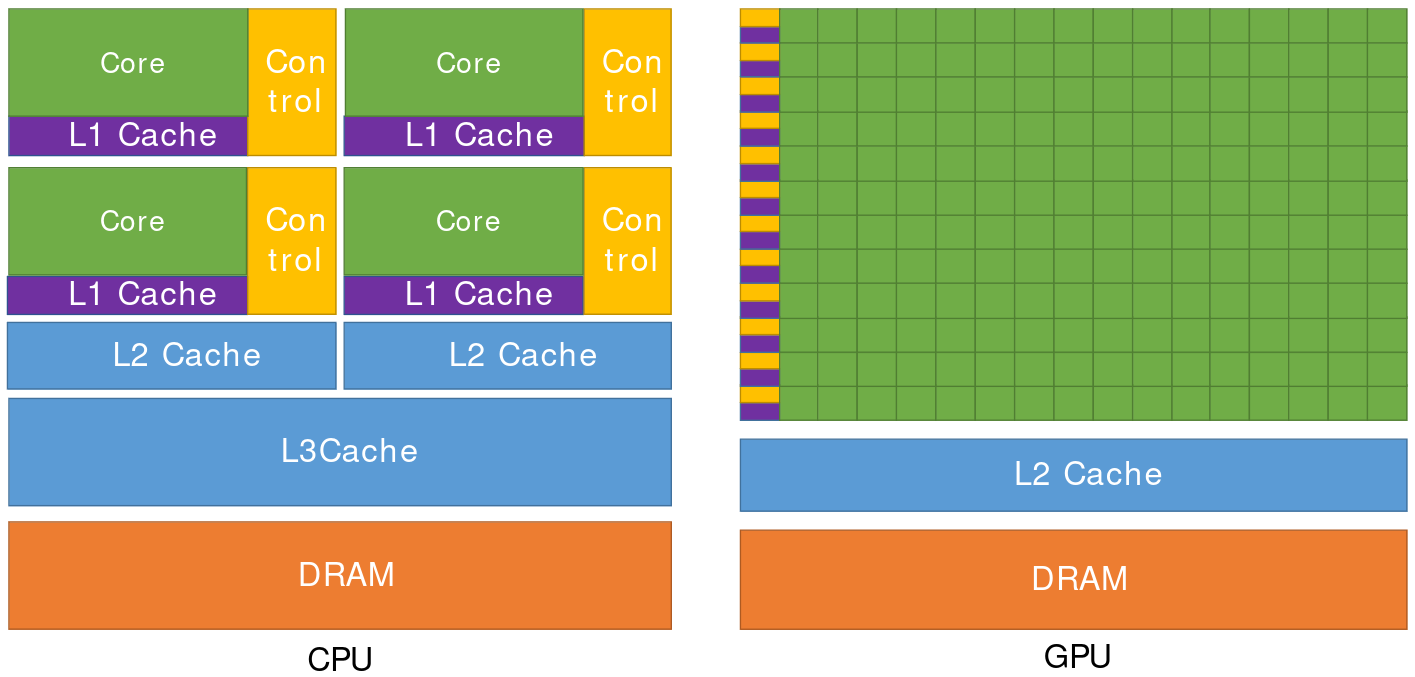
\includegraphics[scale=0.38]{assets/nvidia_die_schema.png}
  \caption{Relative die area usage between a CPU and GPU. Taken from~\cite{nvidia:programming-guide}.}
  \label{fig:gpudiearea}
\end{figure}

The unique workloads that GPU systems handle are characterized by significant spatial locality in memory accesses. Due to this, the caches in GPU systems are generally small as they do not need to frequently cache temporally local values like we do in the CPU. We can procede down the GPU memory hierarchy in the same way we can the CPU hierarchy.

\section{The Register File}

In order to perform latency hiding between multiple warps, each unit of computation (similar to the Vector ALU in a CPU) needs the registers of all the warps that occupy it. This leads to a very large register file. In a RISC-V 32-bit CPU, the register file contains 32 general purpose registers. Each register is 32-bits wide and so the register file is 1024 bits in size. In the MI300X accelerator, the register file is 512 KB in size. This lets us define the occupancy metric for a given compute unit. The occupancy for the MI200 is listed in table~\ref{tab:amdoccupancy}.

\begin{table}
  \centering
  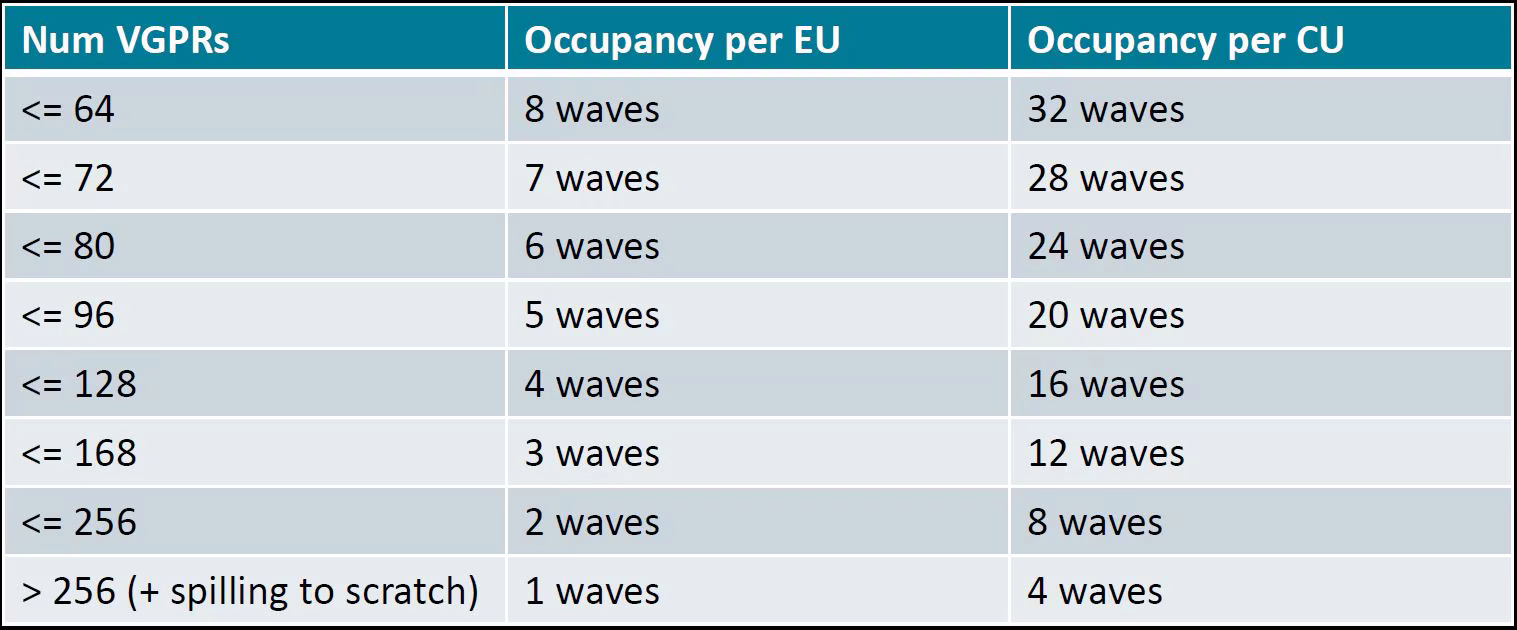
\includegraphics[scale=0.3]{assets/amd_occupancy.png}
  \caption{Occupancy in AMD MI300X accelerators. The occupancy reflects the number of warps that can colocate within a compute unit (CUDA CORE in NVIDIA terms). Taken from~\cite{amd:occupancy, amd:register-pressure}}
  \label{tab:amdoccupancy}
\end{table}

In addition, a study from NVIDIA~\cite{nvidia:register-pressure} shows that modern GPU applications are still limited in registers, but adding more registers does not help performance. This is because as we increase the size of the register file, there is an increased latency to access any individual register.

\section{L1 Cache}

The L1 cache in a GPU contains both the local and shared memory in a given streaming multiprocessor (SM). The L1 in a GPU is banked as well as virtually tagged and virtually addressed, in order to avoid invalidating the entire L1 cache on a context switch~\cite{GPGPUbook} (whenever the GPU switches warps to perform latency hiding). When accessing the cache, a warp will tend to issue many requests at once. In order to not disproportionately affect the bandwidth utilization of any individual unit of computation, the load store units in each unit will perform address coalescing. This coalescing will combine accesses to the same address range in memory into a single request.

L1 cache also serves as a small cache for some data in the global memory (which is generally located in the L2 on the GPU). This is a relatively new development~\cite{nvforum:l1-global-caching}, and certain NVIDIA GPUs will allow for varied models of cache coherency, but in general the L1 cache can store read-only data that is located in the L2 for fast access. There are certain algorithms that benefit from a global memory consistency model~\cite{singh:temporal-coherence}, but these are not the norm in GPU systems.

This L1 cache model is a stark difference from the CPU L1 cache, which is there to cache frequently used values. In general, when we request data from the cache in GPU systems, we will have a cache miss. This is where GPU memory latency hiding, as detailed before, comes in handy. When we make our request, we simply switch to another warp in the queue of possible warps in our compute unit. The latency hiding with gpu systems allows us to avoid waiting for the miss to complete before continuing execution, something we can't do as easily in the CPU since our processor only stores the program state of one program.

\chapter{Issuing a Memory Request}

Please refer to chapter 4 of~\cite{GPGPUbook} for details, as my presentation copies directly from that book.

\chapter{Memory Coherence in GPU systems}

Please refer to reference~\cite{temporalcoherence} for details on the temporal coherence systems currently at the forefront of GPGPU systems research.
